\documentclass[11pt]{article}

\usepackage[margin=1in]{geometry}
\usepackage{amsmath,amssymb}
\usepackage{booktabs}
\usepackage{graphicx}
\usepackage{float}
\usepackage{microtype}
\usepackage{setspace}
\usepackage{natbib}
\usepackage{url}
\usepackage[hidelinks]{hyperref}
\usepackage{caption}
\usepackage{subcaption}
\usepackage{enumitem}

\graphicspath{{figures/}}
\newcommand{\SampleN}{40}
\newcommand{\TestN}{23}
\newcommand{\SampleStart}{January 2015}
\newcommand{\SampleEnd}{October 2024}
\newcommand{\TestStart}{April 2019}
\newcommand{\TestEnd}{October 2024}
\newcommand{\MeanVXAPL}{33.83\%}
\newcommand{\MeanRV}{27.88\%}
\newcommand{\MeanVRP}{0.0328}
\newcommand{\VRPCILow}{0.0150}
\newcommand{\VRPCIHigh}{0.0500}
\newcommand{\VRPPositiveRate}{70.0\%}
\newcommand{\IVSlope}{0.594}
\newcommand{\IVTstat}{2.70}
\newcommand{\IVRsquared}{0.260}
\newcommand{\IVOOSRsquared}{0.115}
\newcommand{\IVRMSE}{0.0666}
\newcommand{\MeanRMSE}{0.0708}
\newcommand{\RidgeRMSE}{0.0696}
\newcommand{\RidgeOOSRsquared}{0.036}
\newcommand{\FiveDayVRP}{-0.0541}


\title{\textbf{Can Earnings Volatility Be Timed?}\\
\large Forecasting Apple's Implied--Realized Variance Spread with Public Data}
\author{[Your Name]\\
\small Independent Quantitative Research Project}
\date{\today}

\begin{document}

\maketitle

\begin{abstract}
This paper examines whether option-implied volatility contains useful information about realized volatility around scheduled corporate earnings announcements, and whether simple public variables improve that forecast. The empirical setting is Apple Inc.\ because the Cboe Apple VIX Index (VXAPL) provides a transparent, model-free measure of 30-day option-implied volatility without requiring a proprietary option-chain database. The sample contains \SampleN\ quarterly announcements from \SampleStart\ through \SampleEnd. Implied variance is compared with annualized realized variance over the following 20 trading days, producing an event-level variance-spread proxy. VXAPL averages \MeanVXAPL, compared with average ex post realized volatility of \MeanRV. The mean implied-minus-realized variance spread is \MeanVRP, with a 95\% event-bootstrap interval of [\VRPCILow, \VRPCIHigh], and is positive in \VRPPositiveRate\ of events. In a full-sample regression, implied variance has a slope of \IVSlope\ ($t_{\mathrm{HC3}}=\IVTstat$) and explains \IVRsquared\ of the variation in subsequent realized variance. In a strict expanding-window exercise covering \TestN\ announcements from \TestStart\ through \TestEnd, an implied-variance-only forecast achieves an out-of-sample $R^2$ of \IVOOSRsquared. A regularized model augmented with recent realized variance, the pre-event VXAPL run-up, and historical earnings-gap magnitude does not materially improve forecast accuracy. The central result is therefore deliberately modest: public option-implied volatility is informative, but a small public dataset does not support a complex timing model. The paper also shows that comparing 30-day implied variance with only five days of realized variance reverses the measured spread, emphasizing the importance of horizon alignment. Because VXAPL is an index rather than a traded option portfolio, all strategy results are presented as variance-payoff proxies, not executable returns.
\end{abstract}

\vspace{0.5em}
\noindent\textbf{Keywords:} implied volatility, realized volatility, variance risk premium, earnings announcements, options, walk-forward testing

\section{Introduction}

Earnings announcements are unusually concentrated information events. A company releases revenue, margins, earnings, guidance, and qualitative information at a known point in time, and the stock price can adjust discontinuously when that information becomes public. Option prices should therefore incorporate not only the background volatility of the stock but also the expected earnings jump. Prior work documents that equity-option implied volatility generally rises before an earnings announcement and falls after the uncertainty is resolved \citep{dubinsky2006earnings,gao2018straddles}. This pattern is intuitive, but it does not by itself answer the economically important question: \emph{was the pre-announcement option-implied variance high enough, too high, or too low relative to what subsequently occurred?}

That question is difficult to answer well with public data. A professional study would normally use a point-in-time option database containing bid and ask quotes, strikes, expirations, open interest, volume, Greeks, and delisting history. Such data allow the researcher to construct delta-hedged option returns, isolate an earnings-specific implied jump, and model the volatility surface. Public sources rarely provide a clean historical surface. A project that silently substitutes today's option chain, uses only surviving contracts, or ignores bid--ask spreads may appear sophisticated while being empirically invalid.

This paper takes a narrower and more defensible approach. It uses the Cboe Apple VIX Index (VXAPL), a VIX-style measure of the market's 30-day expected volatility for Apple stock. Cboe constructs the index from a strip of selected out-of-the-money Apple options and interpolates between near- and next-term maturities to obtain a constant-maturity volatility measure \citep{cboe2025methodology}. VXAPL therefore supplies a public, reproducible option-implied volatility series, although it does not provide individual strike-level information.

The study asks three questions:

\begin{enumerate}[leftmargin=1.5em]
    \item Does pre-announcement VXAPL predict realized variance over the next approximately one month?
    \item Is the event-level implied-minus-realized variance spread positive on average?
    \item Do simple public features improve out-of-sample forecasts beyond implied variance alone?
\end{enumerate}

The design emphasizes research discipline rather than model complexity. All forecast features must be observable at the close of the announcement date, before an after-market earnings release. The contemporaneous realized earnings surprise is excluded from the forecasting model because it is not known at that time. Forecasts are evaluated chronologically using an expanding window; no random train--test split is used. The more complicated model is regularized, and its penalty is fixed rather than selected by searching the test set.

The findings are useful precisely because they are not engineered to produce an impressive backtest. VXAPL contains meaningful forecasting information: its squared value has a positive relation with subsequent realized variance, and the implied-variance-only model modestly beats an expanding historical-mean benchmark out of sample. However, adding a small collection of public features produces little incremental value. The result illustrates a central principle of quantitative research: an economically motivated baseline that survives out-of-sample testing is more credible than a complicated model whose apparent fit does not generalize.

The project contributes in four practical ways. First, it provides a fully reproducible case study using one prepared CSV rather than an opaque data-download pipeline. Second, it distinguishes volatility forecasting from option-profit forecasting. Third, it demonstrates strict information timing and walk-forward evaluation. Fourth, it identifies exactly what additional institutional data would be needed to extend the study: Apple-specific term structure, strike skew, option liquidity, and analyst-dispersion measures.

\section{Institutional Background and Hypotheses}

\subsection{What VXAPL measures}

The Cboe methodology aggregates prices across selected out-of-the-money puts and calls. Each option's contribution depends on its strike spacing, option price, and inverse squared strike; the method then combines near- and next-term variances into a constant 30-day measure \citep{cboe2025methodology}. The resulting index is quoted in annualized volatility points. Thus, an index level of 35 represents approximately 35\% annualized option-implied volatility, and the corresponding annualized implied variance is
\begin{equation}
IV_t = \left(\frac{VXAPL_t}{100}\right)^2.
\end{equation}

The term ``model-free'' should be interpreted carefully. It means that the calculation does not require choosing a particular diffusion model such as Black--Scholes or Heston. It does not mean that the index is free from measurement assumptions. Strike selection, interpolation, stale quotes, bid--ask effects, and the mapping from a finite option strip to expected variance can all matter \citep{jiang2005model}. Nevertheless, a Cboe volatility index is substantially more defensible than using a single at-the-money implied volatility observation.

\subsection{Realized variance and the variance spread}

Following the variance-risk-premium literature, the natural empirical object is the difference between option-implied variance and ex post realized variance \citep{bollerslev2009vrp}. For event date $t$, this study defines 20-trading-day realized variance as
\begin{equation}
RV_{t,t+20}
=
\frac{252}{20}\sum_{j=1}^{20} r_{t+j}^{2},
\qquad
r_{t+j}=\log\left(\frac{P_{t+j}}{P_{t+j-1}}\right),
\end{equation}
where $P_t$ is the split-adjusted closing price. The event-level spread is
\begin{equation}
VRP_t = IV_t - RV_{t,t+20}.
\end{equation}

This quantity is called a variance-spread or variance-risk-premium \emph{proxy}. A true variance-swap payoff requires contract-specific conventions and a replicating option portfolio. Similarly, the return to a short straddle depends on strike, expiration, premium, delta hedging, discrete rebalancing, and transaction costs. None of those objects can be recovered exactly from VXAPL alone. The proxy is still informative because it asks whether the risk-neutral variance embedded in option prices exceeded the physical variance that subsequently occurred.

\subsection{Testable hypotheses}

The first hypothesis concerns information rather than profitability.

\paragraph{H1: Implied variance predicts realized variance.}
If option prices efficiently aggregate market expectations about background and earnings-related uncertainty, the slope coefficient in
\begin{equation}
RV_{t,t+20}=\alpha+\beta IV_t+\varepsilon_t
\end{equation}
should be positive.

\paragraph{H2: The matched-horizon variance spread is positive on average.}
Option sellers may require compensation for bearing volatility and jump risk, while option buyers may be willing to pay for convex protection. These mechanisms imply
\begin{equation}
\mathbb{E}[IV_t-RV_{t,t+20}]>0.
\end{equation}
This need not hold at every event, especially when the earnings jump is unusually large.

\paragraph{H3: Public conditioning variables improve out-of-sample forecasts.}
Recent physical volatility, the run-up in VXAPL, and the magnitude of prior earnings gaps may describe different components of expected risk. A regularized multivariate forecast may therefore improve upon an implied-variance-only model. Because the sample is small, failure to support H3 is a meaningful result rather than a reason to search for more variables.

\section{Data}

\subsection{Sources and sample construction}

The prepared daily CSV combines four components. Apple split-adjusted daily open, high, low, close, and volume observations are sourced from a public repository that identifies Yahoo Finance as the underlying source \citep{aapldataset}. VXAPL, VIX, and VIX9D daily values come from Cboe's historical index files \citep{cboehistorical}. Apple earnings dates and consensus-versus-actual EPS observations are drawn from AlphaQuery, which credits the underlying earnings information to Zacks Investment Research \citep{alphaqueryearnings}.

The daily file covers January 2014 through November 2024. The event sample begins in January 2015 so that rolling features have sufficient history and ends with the October 2024 announcement. It contains \SampleN\ quarterly events. Apple announcements in this period were generally released after the regular close. The forecast is treated as being formed at the close on the listed announcement date, and the first post-announcement close-to-close return is the next trading day's return.

This timing convention prevents a subtle form of look-ahead bias. The actual EPS surprise is retained for descriptive analysis, but it is never used as an ex ante feature. The model may use the average absolute surprise from the \emph{previous} four announcements because those values were already known.

\subsection{Variables}

The main variables are:

\begin{itemize}[leftmargin=1.5em]
    \item \textbf{Implied variance:} squared VXAPL divided by $100^2$.
    \item \textbf{Post-event realized variance:} annualized sum of squared log returns over the next 20 trading days.
    \item \textbf{Pre-event realized variance:} the same measure over the 20 trading days ending on the event date.
    \item \textbf{VXAPL run-up:} percentage change in VXAPL over the previous five trading days.
    \item \textbf{Historical earnings-gap magnitude:} mean absolute overnight close-to-next-open log return across the prior four announcements.
    \item \textbf{Market volatility slope:} $(VIX-VIX9D)/100$, used only in robustness specifications because it is an S\&P 500 rather than Apple-specific term-structure measure.
\end{itemize}

The absence of strike-level data matters. The dataset cannot measure Apple put skew, an Apple-specific volatility term structure, option bid--ask spreads, open interest, or contract-level volume. These are not filled with fabricated proxies. They are treated as omitted variables and motivate future work.

\begin{table}[!htbp]
\centering
\caption{Summary statistics across Apple earnings announcements}
\label{tab:summary}
\begin{tabular}{lrr}
\toprule
Statistic & Mean & Median \\
\midrule
VXAPL implied volatility & 33.83\% & 32.13\% \\
Pre-announcement 20-day realized volatility & 23.07\% & 21.45\% \\
Post-announcement 20-day realized volatility & 27.88\% & 25.43\% \\
Implied variance & 0.1194 & 0.1033 \\
Post-announcement realized variance & 0.0866 & 0.0647 \\
Variance spread $IV-RV$ & 0.0328 & 0.0353 \\
Absolute overnight earnings gap & 3.61\% & 3.42\% \\
\bottomrule
\end{tabular}
\begin{minipage}{0.92\linewidth}
\footnotesize \textit{Notes:} The sample contains 40 quarterly announcements. Volatility is annualized. Implied variance equals $(VXAPL/100)^2$. Realized variance is the annualized sum of squared close-to-close log returns over the next 20 trading days.
\end{minipage}
\end{table}


\section{Empirical Methodology}

\subsection{Descriptive inference}

The average spread is accompanied by a nonparametric 95\% confidence interval obtained from 20,000 event-level bootstrap resamples. Quarterly event windows are sufficiently separated that their 20-day return windows do not overlap. The bootstrap is therefore applied across events rather than across daily observations.

The predictive regression is estimated using ordinary least squares. Because the variance of the residuals may change with the level of volatility, reported standard errors use the HC3 heteroskedasticity correction. The HC3 adjustment is useful in a small sample because it inflates residuals associated with high-leverage observations.

\subsection{Walk-forward forecasting}

Randomly shuffling events would allow future volatility regimes to inform the past and would create an unrealistic estimate of deployable performance. Instead, event $i$ is forecast using only events $1,\ldots,i-1$. The first 16 feature-complete events form the initial estimation window. This produces \TestN\ genuinely out-of-sample forecasts from \TestStart\ through \TestEnd.

Three models are compared:

\begin{enumerate}[leftmargin=1.5em]
    \item \textbf{Historical mean:} the expanding-sample average of realized variance.
    \item \textbf{IV-only OLS:} an expanding regression of realized variance on implied variance.
    \item \textbf{Regularized public-feature model:} ridge regression using implied variance, pre-event realized variance, the five-day VXAPL run-up, and the prior-four-event mean absolute gap.
\end{enumerate}

For the ridge model, predictors are standardized using the training window only. The coefficients solve
\begin{equation}
\widehat{\boldsymbol{\beta}}
=
\arg\min_{\boldsymbol{\beta}}
\left\{
\sum_{s<t}
\left(RV_s-\alpha-\mathbf{x}_s^\top\boldsymbol{\beta}\right)^2
+
\lambda\lVert\boldsymbol{\beta}\rVert_2^2
\right\}.
\end{equation}
The penalty is fixed at $\lambda=10$ to reduce coefficient instability. It is not selected by maximizing test performance. A sensitivity analysis can rerun the specification at $\lambda\in\{0.1,1,10,100\}$.

Forecast performance is reported using mean absolute error, root mean squared error, forecast correlation, and
\begin{equation}
R^2_{\mathrm{OOS}}
=
1-
\frac{\sum_t(RV_t-\widehat{RV}_t)^2}
{\sum_t(RV_t-\overline{RV}_{t,\mathrm{train}})^2}.
\end{equation}
A positive value means the forecast beats the expanding historical-mean benchmark.

\subsection{Economic interpretation}

For each forecast, predicted variance spread is
\begin{equation}
\widehat{VRP}_t=IV_t-\widehat{RV}_t.
\end{equation}
The sign may be interpreted as a hypothetical variance direction: short variance when $\widehat{VRP}_t>0$ and long variance when it is negative. A normalized payoff proxy is
\begin{equation}
\widetilde{\Pi}_t
=
\operatorname{sign}(\widehat{VRP}_t)
\frac{IV_t-RV_t}{IV_t}.
\end{equation}

This is intentionally not called a strategy return. VXAPL itself is not a directly investable Apple variance swap, and the proxy omits option premium financing, vega exposure, delta-hedging error, bid--ask spreads, margin, and tail-risk constraints. Its purpose is to translate forecast direction into an economically interpretable diagnostic, not to claim a realizable Sharpe ratio.

\section{Results}

\subsection{Implied versus realized volatility}

Figure~\ref{fig:ivrvtime} shows that implied and realized volatility move together across broad regimes, including the elevated-volatility period in 2020. VXAPL is not a mechanical forecast of the next 20-day realized volatility: there are announcements after which realized variance is substantially larger than implied variance, and periods when implied volatility remains well above what is subsequently realized.

\begin{figure}[H]
\centering
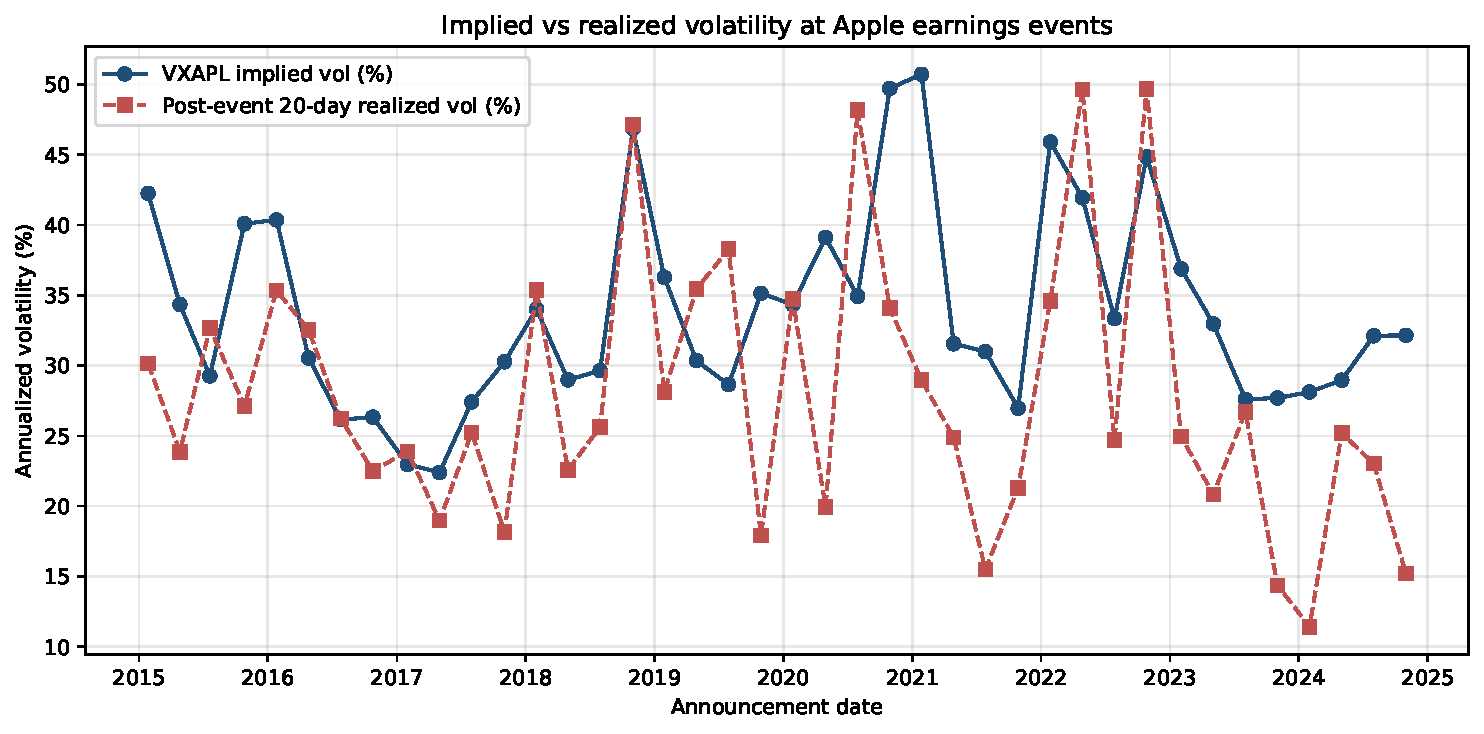
\includegraphics[width=0.95\linewidth]{iv_vs_realized.pdf}
\caption{VXAPL at the earnings-event close and annualized realized volatility over the following 20 trading days.}
\label{fig:ivrvtime}
\end{figure}

Across the \SampleN\ announcements, average VXAPL is \MeanVXAPL, while average post-announcement realized volatility is \MeanRV. The mean variance spread is \MeanVRP, and the event bootstrap places its 95\% interval between \VRPCILow\ and \VRPCIHigh. The spread is positive in \VRPPositiveRate\ of events. These estimates support H2 for the approximately matched horizon, while also showing that short volatility is not a riskless trade.

Figure~\ref{fig:scatter} plots implied variance against realized variance. The positive relation is visible but noisy. A large share of event-specific realized variation remains unexplained, which is expected when one scalar index is used to forecast a path that includes an earnings jump, post-announcement drift, macroeconomic news, and ordinary daily volatility.

\begin{figure}[H]
\centering
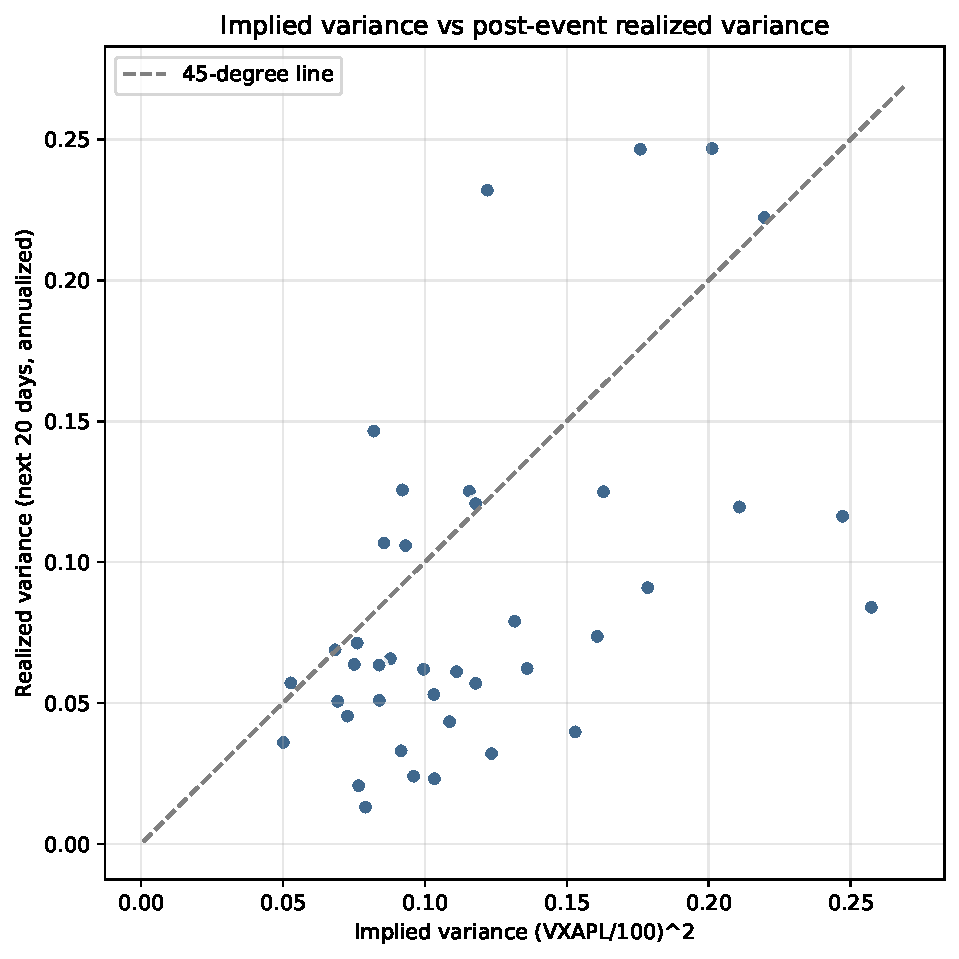
\includegraphics[width=0.72\linewidth]{iv_rv_scatter.pdf}
\caption{Implied variance and subsequent 20-trading-day realized variance. The dashed line is the 45-degree line.}
\label{fig:scatter}
\end{figure}

\subsection{Predictive regressions}

Column (1) of Table~\ref{tab:regression} estimates realized variance using implied variance alone. The slope is \IVSlope\ with an HC3 $t$-statistic of \IVTstat, and the regression explains \IVRsquared\ of realized-variance variation. The coefficient is below one, consistent with implied variance changing more than subsequent realized variance on average, although the small sample does not support a strong structural interpretation of the exact magnitude.

Column (2) adds pre-event realized variance, the five-day VXAPL run-up, and the average absolute earnings gap over the preceding four events. The in-sample $R^2$ rises only slightly. The result cautions against interpreting a longer feature list as better research. In a sample of only a few dozen quarterly observations, additional predictors consume degrees of freedom and can fit noise.

\begin{table}[!htbp]
\centering
\caption{Explaining post-announcement realized variance}
\label{tab:regression}
\begin{tabular}{lcc}
\toprule
 & (1) IV only & (2) Public-feature model \\
\midrule
Intercept & 0.0156 & 0.0197 \\
 & (0.0227) & (0.0415) \\
Implied variance & 0.5944 & 0.7087 \\
 & (0.2205) & (0.3704) \\
Pre-event realized variance &  & -0.1387 \\
 &  & (0.3167) \\
Five-day VXAPL run-up &  & -0.0405 \\
 &  & (0.1380) \\
Prior-four-event mean absolute gap &  & -0.1696 \\
 &  & (0.6486) \\
\midrule
Observations & 40 & 39 \\
$R^2$ & 0.260 & 0.273 \\
\bottomrule
\end{tabular}
\begin{minipage}{0.92\linewidth}
\footnotesize \textit{Notes:} The dependent variable is annualized realized variance over the 20 trading days following the announcement. Parentheses contain HC3 heteroskedasticity-consistent standard errors. The public-feature model excludes the contemporaneous earnings surprise because that value is not known when the forecast is formed.
\end{minipage}
\end{table}


\subsection{Out-of-sample forecasts}

Table~\ref{tab:oos} reports the main walk-forward test. The implied-variance-only model reduces RMSE from \MeanRMSE\ for the expanding-mean benchmark to \IVRMSE, generating $R^2_{\mathrm{OOS}}=\IVOOSRsquared$. This is modest but economically and statistically more credible than an in-sample fit.

The regularized public-feature model records RMSE of \RidgeRMSE\ and $R^2_{\mathrm{OOS}}=\RidgeOOSRsquared$. It does not outperform the IV-only specification. Figure~\ref{fig:wf} illustrates why: the richer model sometimes smooths forecasts, but it does not identify the largest realized-variance events reliably.

\begin{table}[!htbp]
\centering
\caption{Walk-forward out-of-sample forecast performance}
\label{tab:oos}
\begin{tabular}{lrrrr}
\toprule
Model & MAE & RMSE & $R^2_{OOS}$ & VRP sign accuracy \\
\midrule
Expanding historical mean & 0.0580 & 0.0708 & 0.000 & 56.5\% \\
Implied-variance OLS & 0.0551 & 0.0666 & 0.115 & 73.9\% \\
Regularized public-feature model & 0.0600 & 0.0696 & 0.036 & 52.2\% \\
\bottomrule
\end{tabular}
\begin{minipage}{0.92\linewidth}
\footnotesize \textit{Notes:} Every forecast uses only earlier events. $R^2_{OOS}=1-\sum(y-\hat y)^2/\sum(y-\bar y_{train})^2$. The regularized model uses a fixed ridge penalty of 10 after training-sample standardization.
\end{minipage}
\end{table}


\begin{figure}[H]
\centering
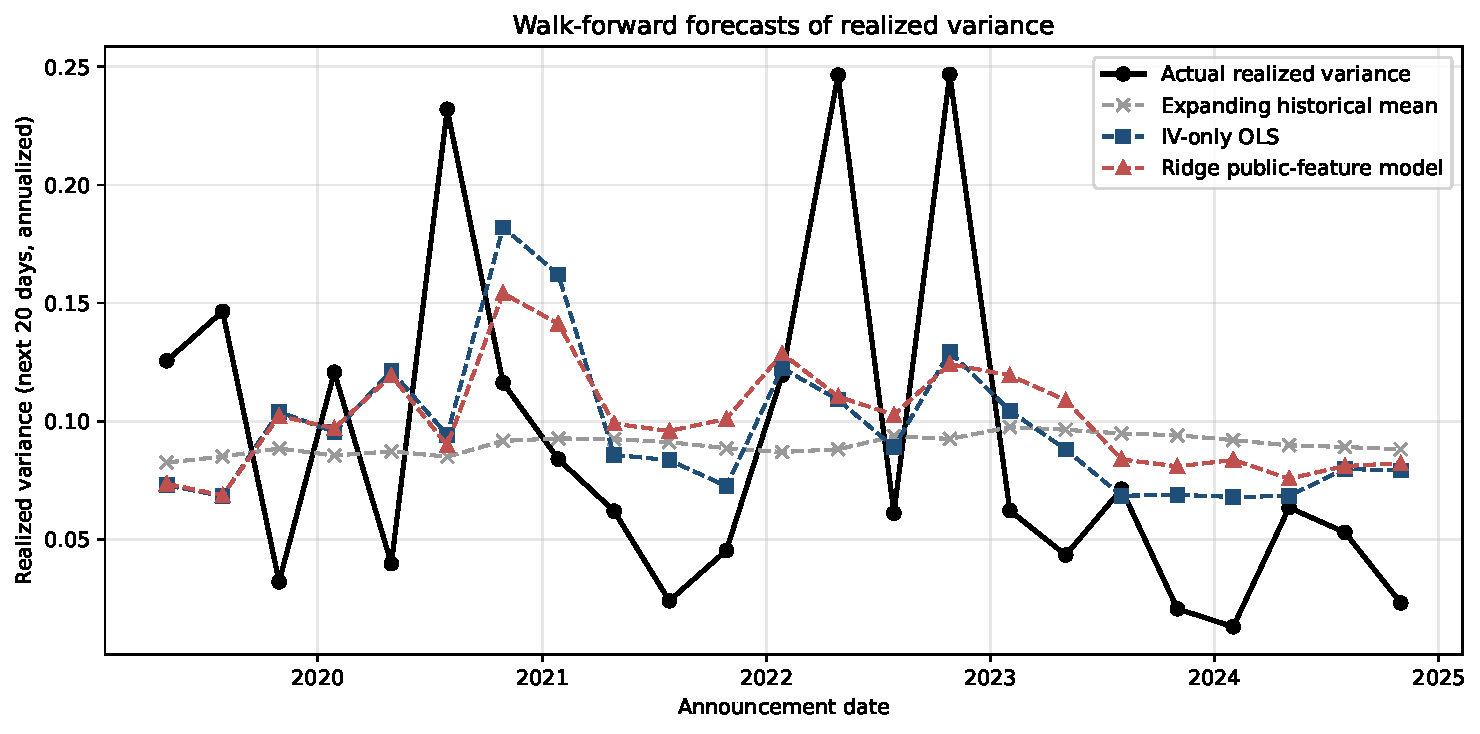
\includegraphics[width=0.95\linewidth]{walk_forward_forecasts.pdf}
\caption{Expanding-window forecasts formed using only prior earnings events.}
\label{fig:wf}
\end{figure}

The IV-only forecast classifies the sign of the realized variance spread correctly in roughly three quarters of the test events. However, this should not be oversold as active timing skill. The model usually predicts a positive spread, which resembles an unconditional short-variance view. The richer model changes direction more often but performs worse. A reasonable interpretation is that the public sample supports estimating the \emph{level} of expected variance more than it supports selecting when to buy versus sell event volatility.

\subsection{Horizon alignment}

The most important robustness result is methodological. VXAPL represents a 30-calendar-day expectation. Comparing it with realized variance over only the first five trading days after earnings creates a horizon mismatch. The five-day window concentrates the earnings jump but discards most of the period priced by VXAPL. As Table~\ref{tab:horizon} shows, the mean spread becomes \FiveDayVRP\ and is positive in only 35\% of events. At the 20-trading-day horizon, the mean spread is positive.

\begin{table}[!htbp]
\centering
\caption{Horizon alignment and the measured variance spread}
\label{tab:horizon}
\small
\begin{tabular}{lrrr}
\toprule
RV horizon & Mean spread & Positive frequency & Interpretation \\
\midrule
5 trading days & -0.0541 & 35.0\% & Event shock dominates \\
20 trading days & 0.0328 & 70.0\% & Approximate horizon match \\
\bottomrule
\end{tabular}
\begin{minipage}{0.92\linewidth}
\footnotesize \textit{Notes:} Both rows use 30-calendar-day VXAPL implied variance. The five-day comparison is deliberately horizon-mismatched and therefore should not be interpreted as a variance risk premium. It is reported to show how the concentrated earnings jump can reverse the sign of the spread.
\end{minipage}
\end{table}


This does not imply that the five-day calculation is wrong; it answers a different question. It asks whether a 30-day implied-volatility index is large relative to an annualized measure dominated by a short earnings shock. The answer is often no. A valid estimate of an earnings-specific premium would require stripping non-event variance from the relevant option maturities or constructing an option strategy whose holding period and expiration match the event window.

Figure~\ref{fig:distribution} shows the full distribution of matched-horizon spreads. The left tail represents the events that make indiscriminate short-volatility strategies dangerous. The positive mean is compensation earned across a distribution with meaningful downside, not an arbitrage.

\begin{figure}[H]
\centering
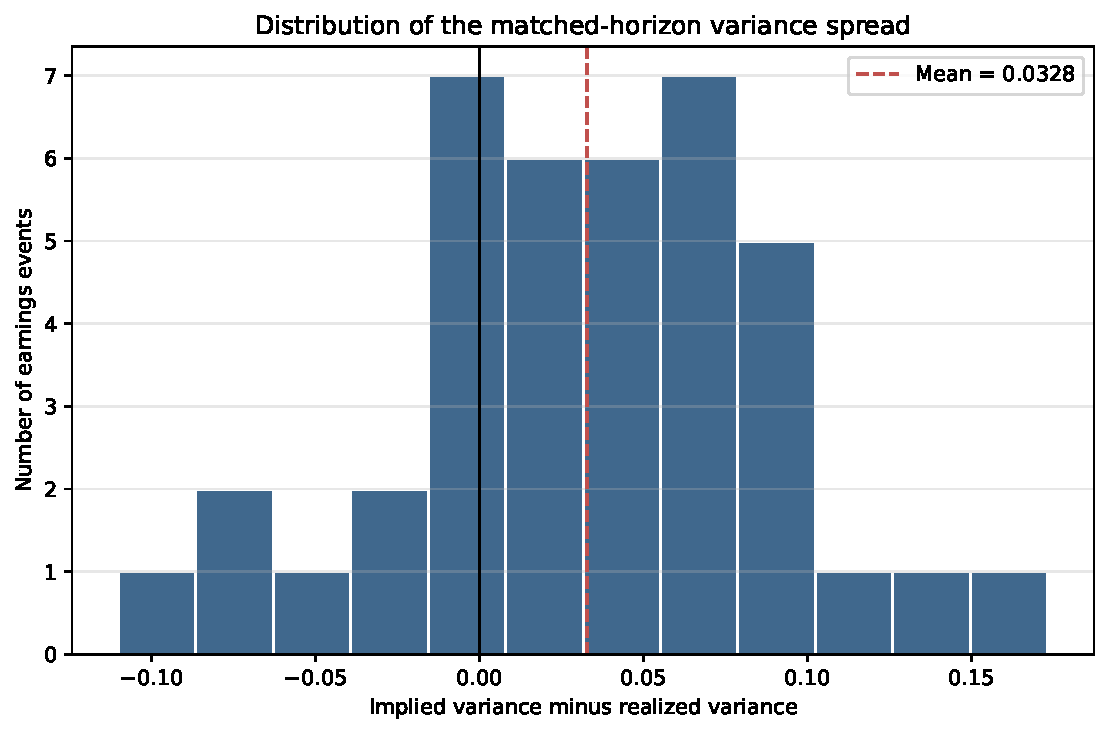
\includegraphics[width=0.72\linewidth]{vrp_distribution.pdf}
\caption{Distribution of the matched-horizon implied-minus-realized variance spread.}
\label{fig:distribution}
\end{figure}

\section{Robustness and Research Integrity}

Several checks are necessary before interpreting the results.

\paragraph{Alternative realized-volatility estimators.}
The baseline uses squared close-to-close returns because those inputs are transparent and robust. Extensions should compare Parkinson range variance, Garman--Klass variance, and realized variance that isolates the close-to-open earnings jump. These estimators answer slightly different questions and should be pre-specified.

\paragraph{Penalty sensitivity.}
The ridge penalty should be varied over a small declared grid. The test sample must not be used to select the winning value. A proper extension would select $\lambda$ within each training window using nested chronological validation, although the small number of events limits the reliability of such tuning.

\paragraph{Influence diagnostics.}
The COVID-19 period and other high-volatility events may have high leverage. The code should report leave-one-event-out estimates, Cook's-distance-style diagnostics, and results excluding 2020. The purpose is not to remove inconvenient observations, but to show whether one regime determines the conclusion.

\paragraph{Timing audit.}
Every feature should include a documented ``known by'' time. Same-day close prices and volatility-index closes are permitted because the decision is formed after the close and before an after-market release. Actual EPS, next-day open, and future realized returns are targets or ex post descriptors only. Unit tests should deliberately perturb future rows and verify that historical features do not change.

\paragraph{Research log.}
All hypotheses, formula choices, horizon definitions, and penalty values should be recorded before viewing the final test results. Failed specifications should remain in the log. This is particularly important in a dataset with only four observations per year, where repeated experimentation can generate attractive but accidental patterns.

\section{Limitations and Institutional Extension}

The principal limitation is not the choice of regression; it is the information set.

First, VXAPL is a constant 30-day volatility index. Earnings announcements affect short-dated options most strongly, so a professional analysis should construct an Apple-specific term structure and estimate the incremental variance assigned to the announcement date. That requires option expirations immediately before and after earnings.

Second, the index aggregates strikes and therefore removes skew. Put skew may contain information about downside jump risk, while smile curvature may reveal a bimodal risk-neutral distribution before earnings. A full surface would allow features such as 25-delta risk reversal, butterfly curvature, and term-specific at-the-money volatility.

Third, the study lacks executable prices. Bid--ask spreads widen around events, and closing midpoints may not be attainable. Contract-level volume and open interest are necessary to screen stale or illiquid quotes. A true backtest should use conservative execution assumptions and report gross and net returns separately.

Fourth, consensus EPS dispersion is unavailable in the public file. The level of disagreement among analysts may be more informative than the consensus estimate itself. Point-in-time IBES data could provide dispersion, revision breadth, and forecast staleness.

Fifth, this is a single-firm case study. Apple is unusually liquid, heavily followed, and may not represent the cross-section. The benefit is clean interpretation; the cost is limited statistical power and external validity.

An institutional extension would use OptionMetrics, CRSP, Compustat, and IBES for a survivorship-bias-controlled universe. It would identify the last tradable option quote before each announcement, construct delta-neutral straddles or model-free variance claims, apply bid--ask and hedging costs, and evaluate results by liquidity, analyst disagreement, earnings uncertainty, skew, and term structure. The public study should be viewed as a transparent prototype of that research design.

\section{Conclusion}

This paper investigates whether public option-implied volatility can forecast realized volatility around Apple earnings announcements. The answer is yes, but with important qualifications. VXAPL contains meaningful information about subsequent 20-day realized variance, and an implied-variance-only model modestly outperforms an expanding historical-mean forecast in a strict walk-forward test. The matched-horizon implied-minus-realized variance spread is positive on average and in most events.

The evidence does not support the claim that a richer public-feature model can reliably time the spread. Recent realized volatility, VXAPL run-up, and historical earnings gaps add little out of sample. Rather than being a disappointing outcome, this is the paper's main research lesson: complexity should earn its place through chronological validation.

The project also demonstrates why volatility studies require precise definitions. A 30-day implied-volatility index compared with a five-day realized window produces a very different spread from a roughly horizon-matched comparison. Likewise, a variance spread is not the same thing as an option return. Clear separation among forecasts, theoretical payoffs, and executable P\&L is essential.

For an application to a quantitative hedge fund, the value of the project is therefore not a claim of discovering a guaranteed trading edge. It is the demonstration of a complete research process: economic motivation, careful information timing, transparent data, reproducible feature construction, robust inference, walk-forward testing, honest failure of a more complex model, and a precise roadmap for improving the analysis with institutional data.

\begin{thebibliography}{99}

\bibitem[Bollerslev et al.(2009)]{bollerslev2009vrp}
Bollerslev, T., Tauchen, G., and Zhou, H. (2009).
Expected stock returns and variance risk premia.
\emph{The Review of Financial Studies}, 22(11), 4463--4492.

\bibitem[Cboe Global Markets(2025)]{cboe2025methodology}
Cboe Global Markets (2025).
\emph{Volatility Index Methodology: Selected Broad-Based Index, Equity and ETF Volatility Indices}.
Available from Cboe Global Indices.

\bibitem[Cboe Global Markets(2026)]{cboehistorical}
Cboe Global Markets (2026).
\emph{Historical Data for Cboe VIX Index and Other Volatility Indices}.
Accessed June 2026.

\bibitem[Dubinsky and Johannes(2006)]{dubinsky2006earnings}
Dubinsky, A. and Johannes, M. (2006).
Earnings announcements and equity options.
Working paper, Columbia Business School.

\bibitem[Gao et al.(2018)]{gao2018straddles}
Gao, G. P., Xing, Y., and Zhang, X. (2018).
Anticipating uncertainty: Straddles around earnings announcements.
\emph{Journal of Financial and Quantitative Analysis}, 53(6), 2587--2617.

\bibitem[Goyal and Saretto(2009)]{goyal2009options}
Goyal, A. and Saretto, A. (2009).
Cross-section of option returns and volatility.
\emph{Journal of Financial Economics}, 94(2), 310--326.

\bibitem[Jiang and Tian(2005)]{jiang2005model}
Jiang, G. J. and Tian, Y. S. (2005).
The model-free implied volatility and its information content.
\emph{The Review of Financial Studies}, 18(4), 1305--1342.

\bibitem[Market Computing(2026)]{alphaqueryearnings}
Market Computing, LLC (2026).
Apple Inc. earnings history.
Underlying earnings data credited by the provider to Zacks Investment Research.

\bibitem[Ali(2024)]{aapldataset}
Ali, F. (2024).
Apple AAPL stock data 1980 to December 2024.
Public Apache-2.0 repository using Yahoo Finance data.

\end{thebibliography}

\appendix

\section{Reproducibility Checklist}

\begin{enumerate}[leftmargin=1.5em]
    \item Read only \texttt{data/aapl\_earnings\_volatility\_data.csv}; make no network requests.
    \item Parse dates and sort observations before calculating any rolling statistic.
    \item Calculate log returns from the adjusted close supplied in the file.
    \item Form all event features using rows at or before the announcement-date close.
    \item Calculate realized-variance targets using only rows after the event.
    \item Use expanding-window forecasts; never shuffle event observations.
    \item Standardize ridge predictors using training-window moments only.
    \item Save event-level predictions so every figure and table can be audited.
    \item Label normalized variance payoffs as proxies rather than option returns.
    \item Preserve a research log containing all attempted specifications.
\end{enumerate}

\section{Core Formula Summary}

\begin{align}
r_t &= \log(P_t/P_{t-1}),\\
IV_t &= (VXAPL_t/100)^2,\\
RV^{(h)}_t &= \frac{252}{h}\sum_{j=1}^{h}r_{t+j}^2,\\
VRP^{(h)}_t &= IV_t-RV^{(h)}_t,\\
R^2_{\mathrm{OOS}}&=1-\frac{\sum_t(y_t-\widehat y_t)^2}
{\sum_t(y_t-\bar y_{t,\mathrm{train}})^2}.
\end{align}

\end{document}
